\documentclass[12pt,a4paper]{article}

\usepackage[utf8]{inputenc}
\usepackage[T2A]{fontenc}
\usepackage[russian]{babel}
\usepackage[margin=2.3cm]{geometry}
\usepackage{amsmath,amssymb}
\usepackage{booktabs}
\usepackage{longtable}
\usepackage{array}
\usepackage{graphicx}
\usepackage{xcolor}
\usepackage{url}
\urlstyle{tt}
\usepackage{caption}
\usepackage{enumitem}
\usepackage[colorlinks=true,linkcolor=blue!50!black,urlcolor=blue!50!black,citecolor=blue!50!black]{hyperref}

\sloppy
\setlist{itemsep=2pt,topsep=4pt}
\renewcommand{\arraystretch}{1.15}
\captionsetup{font=small,labelfont=bf}
\graphicspath{{figures/}}

\newcommand{\rhoJ}{\rho J}
\newcommand{\kT}{k_BT}

\title{Отчёт о работе после замечаний от 10.10.2026 A.Е Теретёнкова и симуляции статей по Kondo}
\date{19.11.2026}

\begin{document}
\maketitle

Отчёт о работе после письма А.~Е.~Теретенкова от 10.10.2026 с замечаниями к постановке задачи.
Раздел~\ref{sec:remarks} --- замечания из письма и что по каждому сделано; раздел~2 --- моделирование двух
статей Delgado и симулятор; разделы 3--6 --- остальная работа.
Числа взяты из файлов репозитория (\texttt{experiments/results/r28/},
\path{paper/report_2026-11/numbers.json}) или посчитаны скриптами
\path{paper/report_2026-11/make_figures.py}, \path{digitize_reference.py} и \path{kondo_demo.py}.
Результаты, не повторённые на нескольких выборках, помечены как предварительные.

\section{Замечания А.~Е.~Теретенкова и что по ним сделано}\label{sec:remarks}

По оценке письма физическая модель (уравнение Линдблада, $\gamma(t)$) и часть с прогнозом корректны;
замечания относятся к модели наблюдения --- к тому, какие входы доступны в эксперименте. Замечания
записаны в \path{notes/plan_2026-10.md}, §3; там же план исправлений (§5: A --- тексты, B --- расчёты,
C --- новое направление).

{\small\noindent\begin{longtable}{p{4.4cm}p{5.4cm}p{4.6cm}}
\toprule
Замечание & Сделано & Не сделано \\
\midrule
1. Входы --- точные ансамблевые средние из $\rho(t)$; в эксперименте есть только исходы 0/1 отдельных
измерений, средние получаются из многих повторных приготовлений, измерение меняет состояние. &
Модель наблюдения с конечным числом повторов $N$ (раздел~3): оценки средних из выборки исходов,
когерентность и чистота из тех же оценок. В поздних R29/R30 модели обучены и проверены на таких
входах; первичные CSV и параметры сведены в отдельном отчёте
\path{output/pdf/decoherence_study.pdf}. Симулятор последовательных проективных измерений
с коллапсом (раздел~4). &
Модели и цели на записях одного экземпляра нет; аппаратная проверка не проведена. \\
2. Для двух кубитов когерентность и чистота --- глобальные величины, шести локальных средних для них
мало; базовый набор фактически требует томографии; «частичное наблюдение» в статье~2 названо неверно. &
Режимы измерения разделены: \texttt{local} (3 настройки) даёт шесть локальных средних без когерентности
и чистоты, \texttt{tomography} (9 настроек) --- корреляторы, когерентность и чистоту.
R30 сравнивает эти входы; статья~2 исправлена в текстовой ветке и перенесена в рабочую копию. &
Локальный результат BiLSTM в R30 требует исправления входных скаляров и повтора запуска. \\
3. Время набора данных (повторы $\times$ настройки $\times$ моменты окна) не оценено и больше
прогнозируемого остатка. &
Формула стоимости и пример (раздел~3), таблицы R29/R30 в отдельном отчёте. &
Аппаратная длительность приготовления, эволюции и считывания не измерена; сравнение времени
набора с прогнозируемым остатком открыто. \\
4. Сценарий «предупреждение во время вычисления» (online, QEC scheduler, real-time) не обоснован. &
Статья~1 и русское описание переписаны для ансамблевой характеризации и калибровки;
утверждения об online-предупреждении и управлении одним работающим кубитом сняты. &
Применимость к аппаратному циклу требует отдельного опыта. \\
5. В обзоре не хватает работ \cite{luchnikov2020,teretenkov2026,mavadia2017,maan2026,napdd2026};
сравнение с \cite{chenkuo2025} не касается доступности входов. &
Работы разобраны в \path{notes/literature_advisor_2026-10.md}, добавлены в обе статьи и
\texttt{description\_ru.tex}; сравнение с \cite{chenkuo2025} уточняет доступность входов. &
Подробная проверка дополнительных материалов Luchnikov et al. и разделов III/V
Teretenkov et al. остаётся в плане. \\
\midrule
Новое направление (C): вход --- запись последовательных измерений одного экземпляра,
обучение генератора по правдоподобию записи \cite{luchnikov2020}, связь с ограниченными наблюдаемыми
\cite{teretenkov2026}. &
Симулятор записей (раздел~4). &
Базовая модель по правдоподобию, цель на записях, обнаружение дрейфа $\gamma$. \\
\bottomrule
\end{longtable}}

Попутно была найдена ошибка во введении статьи~1: числа одного прогона E5.
В новой редакции они заменены результатами повторов.

Вне замечаний: микроскопический диссипатор (ванна Кондо) со сравнением с напечатанными рисунками и
демонстрацией на двух кубитах (раздел~2); блочный конструктор, экран сборки рецептов в интерфейсе и
порядок в экспериментах (раздел~5).

\clearpage
\section{Микроскопическая модель диссипации: ванна Кондо}

\subsection{Модель}

Локализованные спины в точках $\mathbf r_l$ связаны обменом с газом свободных электронов
размерности $d$: $V=J\sum_l \mathbf S_l\cdot\mathbf s(\mathbf r_l)$. В
втором порядке по $\rhoJ$ и в секулярном (Davies) пределе уравнения Блоха--Рэдфилда
скорость перехода между собственными состояниями $|M\rangle$ гамильтониана спинов $H$ ($\hbar=1$)
\begin{equation}
\Gamma(M\to M')=\frac{\pi(\rhoJ)^2}{4}\,G(E_M-E_{M'})
\sum_{l,l'}K_d\!\big(k_F|\mathbf r_l-\mathbf r_{l'}|\big)
\sum_a\langle M'|S^a_l|M\rangle\langle M|S^a_{l'}|M'\rangle,
\label{eq:rate}
\end{equation}
\begin{equation}
G(\Delta)=\frac{\Delta}{1-e^{-\Delta/\kT}},\quad G(0)=\kT,\qquad
K_1=\cos^2x,\quad K_2=J_0^2(x),\quad K_3=\Big(\frac{\sin x}{x}\Big)^2 .
\end{equation}
Это PRB~95, 075413 (ур.~12--13, 20, 26, 31--34) и Surf.\ Sci.\ 630, 337 (ур.~14--16)
\cite{delgado2017,delgado2014}; префактор $\pi/4$ взят из ур.~20 PRB. Параметры
модели: $\rhoJ$, $\kT$, $k_Fd$.

Для динамики матрица ядра диагонализуется, $K_{ll'}=\sum_c\lambda_c u_c(l)u_c(l')$, и вводятся
коллективные операторы $A_{c,a}=\sum_l u_c(l)S^a_l$. Каждый раскладывается по боровским частотам,
$A_{c,a}(\omega)=\sum_{E_M-E_{M'}=\omega}|M'\rangle\langle M'|A_{c,a}|M\rangle\langle M|$, и
\begin{equation}
L_{c,a,\omega}=\sqrt{\tfrac{\pi(\rhoJ)^2}{4}\,\lambda_c\,G(\omega)}\;A_{c,a}(\omega)
\end{equation}
--- операторы коллапса для \texttt{qutip.mesolve}. Часть $\omega=0$ даёт чистую дефазировку со скоростью
$\propto\kT$. Скорость затухания когерентности между $M$ и $M'$ (PRB, ур.~14--15):
$1/T_2=\gamma^{\rm ad}+\tfrac12(\sum_N\Gamma_{M\to N}+\sum_N\Gamma_{M'\to N})$,
\begin{equation}
\gamma^{\rm ad}_{MM'}=\tfrac12\cdot\tfrac{\pi(\rhoJ)^2}{4}\,\kT\sum_a\sum_{ll'}K_{ll'}\,
\Delta S^a_l\,\Delta S^a_{l'},\quad \Delta S^a_l=\langle M|S^a_l|M\rangle-\langle M'|S^a_l|M'\rangle .
\end{equation}
При точном вырождении уровней скорости между отдельными состояниями зависят от выбора базиса внутри уровня;
операторы коллапса от этого выбора не зависят. Сдвиг уровней (Lamb shift) посчитан отдельно, в динамику не добавлен.
Реализация: \path{src/physics/kondo_bath.py}; предупреждение при $\rhoJ>0.3$.

\subsection{Как модель входит в симулятор}\label{sec:model}

Кубиты --- спины $S=1/2$, $\mathbf S=\boldsymbol\sigma/2$, в точках $0$ и $d$ на прямой; $H$ задан
паулиевскими матрицами (XXZ: $J(XX+YY+ZZ)$, то есть изотропный случай $\Delta=1$; TFIM: $J\,XX+Z_1+Z_2$). Параметры модели --- $\rhoJ$, $\kT$ и
$k_Fd$ --- в единицах $H$ ($\hbar=1$). В блоке \texttt{channels.kondo\_bath} $k_F=1$, а расстояние
задаёт параметр \texttt{spacing}: положения спинов умножаются на него, так что ядро $K_d$ видит
$k_F|\mathbf r_1-\mathbf r_2|=k_Fd$.

Каналы Кондо заменяют феноменологические каналы $\sigma^-$ и $\sigma^z$ со скоростью $\gamma(t)$:
вместо одного оператора на кубит блок возвращает набор операторов коллапса со скоростями внутри
(в проверке ниже, для $d=2$, $k_Fd/\pi=0.5$, их 9). Остальные стадии рецепта (начальное состояние,
наблюдаемые, цель) не меняются, поэтому цель, например $T_2^E$, считается тем же блоком
\texttt{target}. Рецепт демонстрации из п.~\ref{sec:demo}:

\begin{verbatim}
Recipe(system=block("system.two_qubit", J=0.8, interaction="XXZ"),
       channels=(block("channels.kondo_bath", rho_J=0.1, kT=0.2, k_F=1.0,
                       dim=2, spacing=math.pi * 0.5),),  # k_F d/pi=0.5
       initial=block("initial.random_pure"),
       observe=(block("observe.purity"),),
       target=block("target.energy_basis_crossing", threshold=1 / math.e),
       t_max=1200.0, dt=1.0)
\end{verbatim}

Зависимость от времени. После каналов Кондо можно поставить \texttt{channels.bernstein\_profile}
(или \texttt{channels.ou\_modulation}): модификатор умножает скорости всех предшествующих каналов на
$\gamma(t)$, то есть $(\rhoJ)^2\to(\rhoJ)^2\gamma(t)$. Проверка (\path{paper/report_2026-11/kondo_demo.py},
XXZ, $d=2$, $k_Fd/\pi=0.5$, $t_{\max}=1200$, $dt=1$, одно начальное состояние): с постоянными
коэффициентами $(c,c,c)$ коэффициенты QuTiP равны $\sqrt c$ с отклонением
$\le2.2\cdot10^{-16}$. $T_2^E$ с профилем: 222.5 при $c=0.5$ и 55.6 при $c=2$; без профиля 111.2.
Относительное расхождение с $T_2^E$ при всех скоростях, умноженных на $c$: $4.6\cdot10^{-4}$ и
$7.4\cdot10^{-14}$; с $T_2^E(1)/c$: $8.7\cdot10^{-5}$ и $9.3\cdot10^{-5}$ (\path{numbers_kondo_demo.json},
\texttt{bernstein\_check}). Это согласуется с масштабированием $1/c$ в пределах ошибки интерполяции
пересечения. Проверены только постоянные коэффициенты; непостоянный профиль на каналах Кондо, модуляция OU
здесь и применимость секулярной формы к меняющемуся во времени $\rhoJ$ не проверялись.

Условия применимости для выбранных параметров (табл.~\ref{tab:validity}, максимум по сетке
$k_Fd/\pi\in[0,2]$, $d=1,2,3$ из п.~\ref{sec:demo}).
\begin{itemize}
\item Борновское приближение: $\rhoJ=0.1\ll1$ (код предупреждает при $\rhoJ>0.3$).
\item Секулярное приближение: наибольшая скорость $\Gamma_{\rm dec}^{\max}$ (максимум из
суммарных скоростей ухода из состояний и скоростей затухания когерентностей между невырожденными
уровнями) против наименьшего ненулевого расстояния $\Delta_{\min}$ между различными боровскими частотами.
Отношение $\le0.0044$ для XXZ и $\le0.0944$ для TFIM (максимум при $k_Fd=0$); наибольшая скорость отдельного
перехода даёт $\le0.0039$ и $\le0.0943$. Условие выполнено везде на сетке; для TFIM запас около одного порядка.
Сравнение с уравнением Блоха--Рэдфилда без секулярного приближения не делалось.
\item Марковость: $\Gamma_{\rm dec}^{\max}/\kT\le0.12$; время корреляции ванны порядка $1/\kT$, а
$\kT\cdot T_2^E\ge20.6$ на всей сетке.
\item $\Gamma_{\rm dec}^{\max}T_2^E=1.44$--$1.49$ (XXZ) и $1.97$--$2.74$ (TFIM): $T_2^E$ составляет
от 1.4 до 2.7 обратной наибольшей скорости, то есть затухание происходит за одно--три характерных времени, а не
за много.
\end{itemize}

\paragraph{Секулярное и несекулярное уравнение.} Исключение ванны во втором порядке по $\rhoJ$ в
марковском пределе даёт уравнение Блоха--Рэдфилда; в собственном базисе $H$
\begin{equation}
\dot\rho_{ab}=-i\omega_{ab}\rho_{ab}+\sum_{cd}R_{ab,cd}\,\rho_{cd},\qquad \omega_{ab}=E_a-E_b .
\end{equation}
Тензор $R$ связывает все элементы $\rho$: заселённости с когерентностями и когерентности между собой.
Слагаемое $R_{ab,cd}\rho_{cd}$ с $\omega_{cd}\ne\omega_{ab}$ осциллирует как $e^{i(\omega_{ab}-\omega_{cd})t}$ и за
время релаксации почти усредняется, если $|\omega_{ab}-\omega_{cd}|\gg\Gamma$. Секулярное приближение
отбрасывает такие слагаемые и оставляет только пары с равными частотами. Тогда заселённости подчиняются
кинетическому уравнению со скоростями~\eqref{eq:rate}, каждая когерентность затухает со своей
скоростью $1/T_2$, а генератор имеет форму Линдблада (ГКСЛ), что гарантирует положительность $\rho$.
Так устроены операторы $L_{c,a,\omega}$: разные боровские частоты в них не смешиваются.
Несекулярное уравнение сохраняет полный тензор $R$; оно точнее, когда расстояния между частотами
сравнимы со скоростями, но в общем случае не имеет формы ГКСЛ и может нарушать положительность.
Приведённое выше отношение $\Gamma_{\rm dec}^{\max}/\Delta_{\min}$ --- как раз мера применимости
секулярного приближения. Для TFIM (до 0.094) сравнение с несекулярным уравнением показало бы, насколько
приближение меняет $T_2^E$; тензор $R$ строится из тех же матричных элементов, что уже вычисляются.

\begin{table}[h]
\centering\small
\begin{tabular}{lcccccc}
\toprule
& $\Delta_{\min}$ & $\Gamma_{\rm tr}^{\max}$ & $\Gamma_{\rm dec}^{\max}$ & $\Gamma_{\rm dec}^{\max}/\Delta_{\min}$ & $\Gamma_{\rm dec}^{\max}/\kT$ & $\Gamma_{\rm dec}^{\max}T_2^E$ \\
\midrule
XXZ & 3.200 & 0.0126 & 0.0141 & 0.0044 & 0.071 & 1.44--1.49 \\
TFIM & 0.246 & 0.0232 & 0.0232 & 0.0944 & 0.116 & 1.97--2.74 \\
\bottomrule
\end{tabular}

\caption{Проверка параметров $\rhoJ=0.1$, $\kT=0.2$, $J=0.8$ по сетке п.~\ref{sec:demo}. $\Gamma_{\rm tr}^{\max}$ ---
наибольшая скорость перехода между собственными состояниями, $\Gamma_{\rm dec}^{\max}$ --- наибольшая
скорость затухания, $\Delta_{\min}$ --- наименьшее ненулевое расстояние между различными боровскими частотами.}
\label{tab:validity}
\end{table}

\subsection{Проверки реализации}

\begin{itemize}
\item \textbf{Предел Корринги, один спин $1/2$.} $\Gamma=\pi(\rhoJ)^2G(\Delta)/8$ (SS ур.~14, PRB ур.~22).
При $\Delta\gg\kT$ скорость линейна по $\Delta$; при $\Delta/\kT=0.01$
$\Gamma/(\pi(\rhoJ)^2\kT/8)=1.005$, 0.5\% --- первый член разложения $G=\kT(1+\Delta/2\kT)$
(\path{deviations_surf.csv}).
\item \textbf{Детальный баланс и состояние Гиббса.} $G(-\Delta)=G(\Delta)e^{-\Delta/\kT}$, стационарное
состояние лиувиллиана --- гиббсово состояние $H$ (тесты \path{test_rates_obey_detailed_balance...},
\path{test_steady_state_is_the_gibbs_state}).
\item \textbf{Лиувиллиан операторов коллапса} в собственном базисе $H$ воспроизводит скорости
заселённостей и $1/T_2$ с точностью $\le10^{-14}$ (случайные трёхспиновые цепочки Гейзенберга в
случайных полях, $d=1,2,3$; тест \path{test_collapse_dynamics_reproduce_rates_and_dephasing}).
Поэтому проверки скоростей ниже относятся и к тому, что интегрирует симулятор.
\end{itemize}

\subsection{Воспроизведение результатов статей}

Скрипт \path{experiments/new/r28_kondo_reproduction.py}; максимальные отклонения в
\path{deviations_*.csv} (табл.~\ref{tab:dev}). Значения $\sim10^{-15}$ --- машинная точность, не измерение.
Рис.~\ref{fig:dimer} и~\ref{fig:surf} скопированы из \texttt{experiments/results/r28/}, рис.~\ref{fig:sw}
перестроен из CSV того же каталога (\path{make_figures.py}). Сравнение с напечатанными кривыми ---
п.~\ref{sec:digitize}.

\begin{figure}[h]
\centering
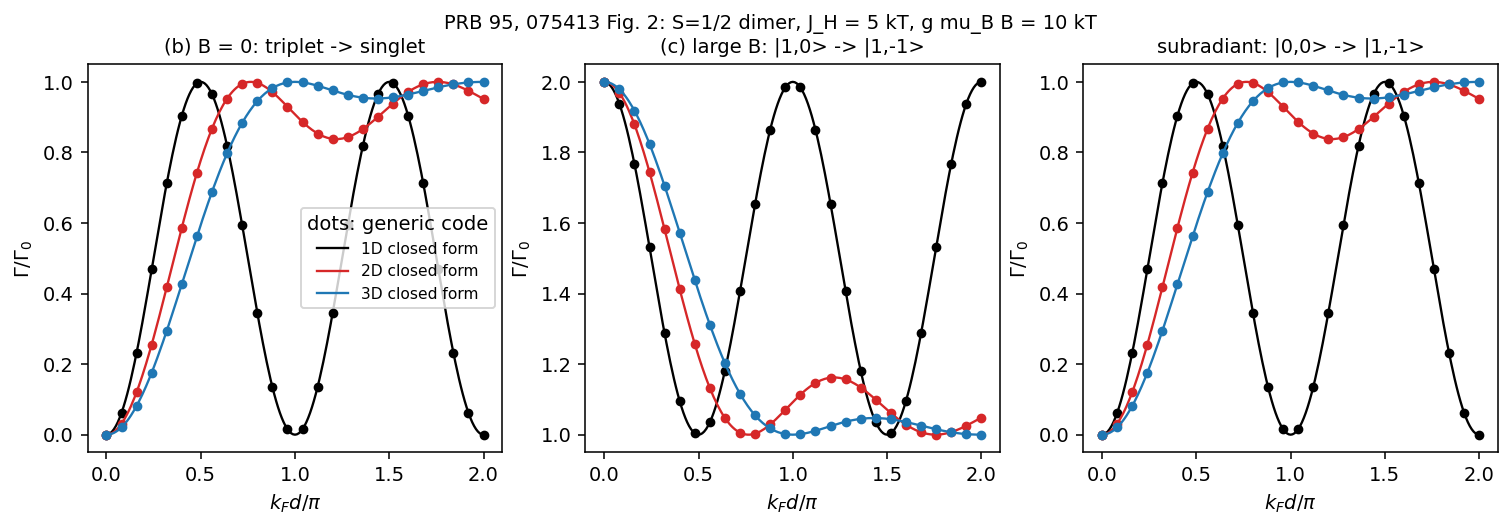
\includegraphics[width=\textwidth]{fig2_dimer.png}
\caption{PRB рис.~2: димер $S=1/2$, $J_H=5\kT$. Точки --- общий код, линии --- замкнутые формы
$1-K_d$ и $1+K_d$ (панель (b): ур.~31--32, наш расчёт; см.\ расхождение (i)).}
\label{fig:dimer}
\end{figure}

\paragraph{Рис.~3 PRB (цепочка $S=3/2$, $D=J_H=-1$ мэВ, 3D-газ).} $H$ строится на секторах $S_z=3N/2$ и
$3N/2-1$. Ур.~37, $\Gamma_{SW1}(N)/\Gamma_{SW1}(1)=N$, выполнено с отклонением $\le8\cdot10^{-15}$ для
$N=4,5,6,8$. SW2 не распадается при $k_Fd=0$. Максимумы SW2: $N=4$: 1.83 при $k_Fd/\pi=0.375$;
$N=5$: 2.01 при 0.275; $N=6$: 2.23 при 0.25; $N=8$: 2.74 при 0.175 (\path{numbers.json},
\texttt{fig3\_sw2\_peaks}). Для $N=8$ в статье на глаз около 2.7 при около 0.2; остальные значения статьи
не считывались.

\paragraph{Рис.~4 PRB (цепочки Изинга, $k_Fd/\pi=0.01$).} $\Lambda=4s^{T}Ks$, $s_l=\pm1$;
проверка по \path{kondo_rates} на полном пространстве $2^N$, $N=2..8$: отклонение $\le5.7\cdot10^{-14}$.

\begin{figure}[h]
\centering
\begin{minipage}[t]{0.55\textwidth}
\centering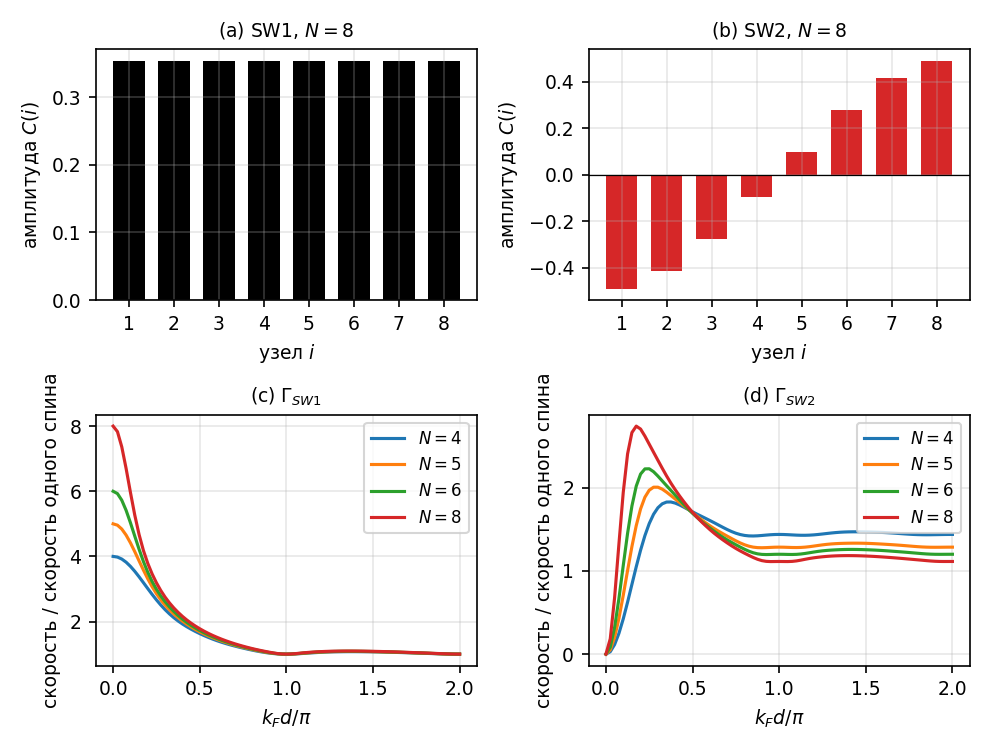
\includegraphics[width=\textwidth]{fig3_spin_waves_report.png}
\end{minipage}\hfill
\begin{minipage}[t]{0.40\textwidth}
\centering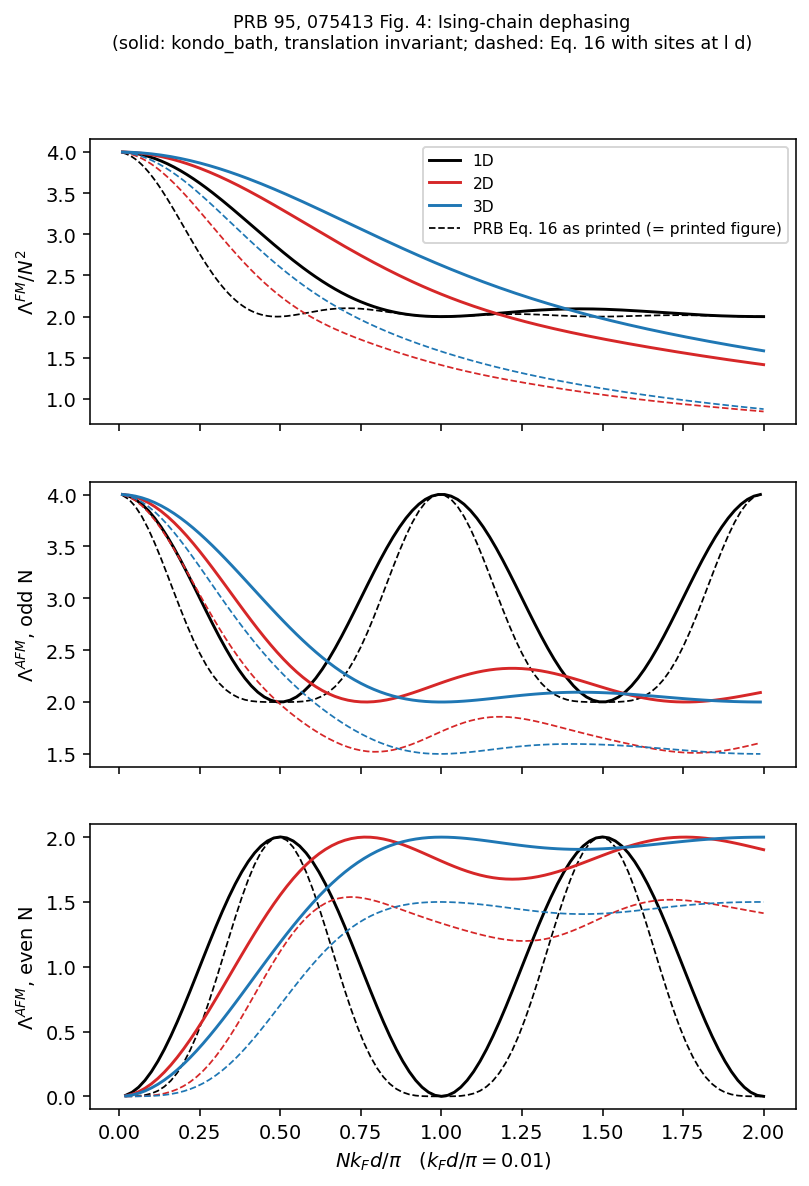
\includegraphics[width=\textwidth]{fig4_ising_dephasing.png}
\end{minipage}
\caption{Слева: PRB рис.~3. Справа: PRB рис.~4; сплошные --- трансляционно-инвариантная форма
(\texttt{kondo\_bath}), пунктир --- ур.~16 как напечатано (воспроизводит рисунок статьи).}
\label{fig:sw}
\end{figure}

\paragraph{Surf.\ Sci.} Ур.~15 против квадратуры $f(\epsilon)(1-f(\epsilon+\Delta))$ при $\Delta/\kT\in[-6,12]$:
$2.6\cdot10^{-13}$. Ур.~21 против независимого расчёта той же суммы: $2\cdot10^{-16}$. Ур.~22
(спин $1/2$) воспроизводится; ур.~23 и 24 --- нет (расхождение (v)).

\begin{figure}[h]
\centering
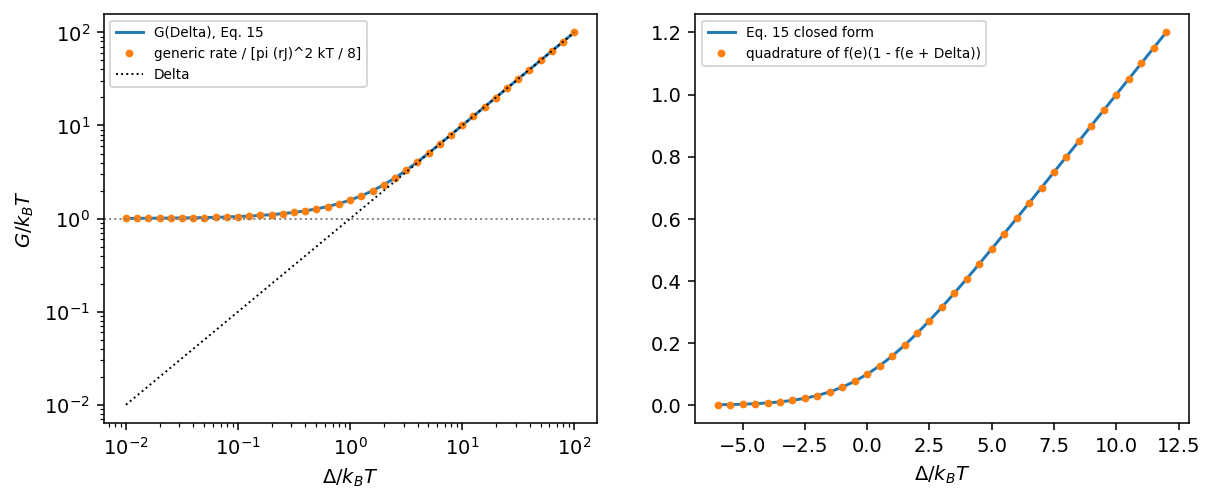
\includegraphics[width=0.48\textwidth]{fig_surfsci_korringa.png}\hfill
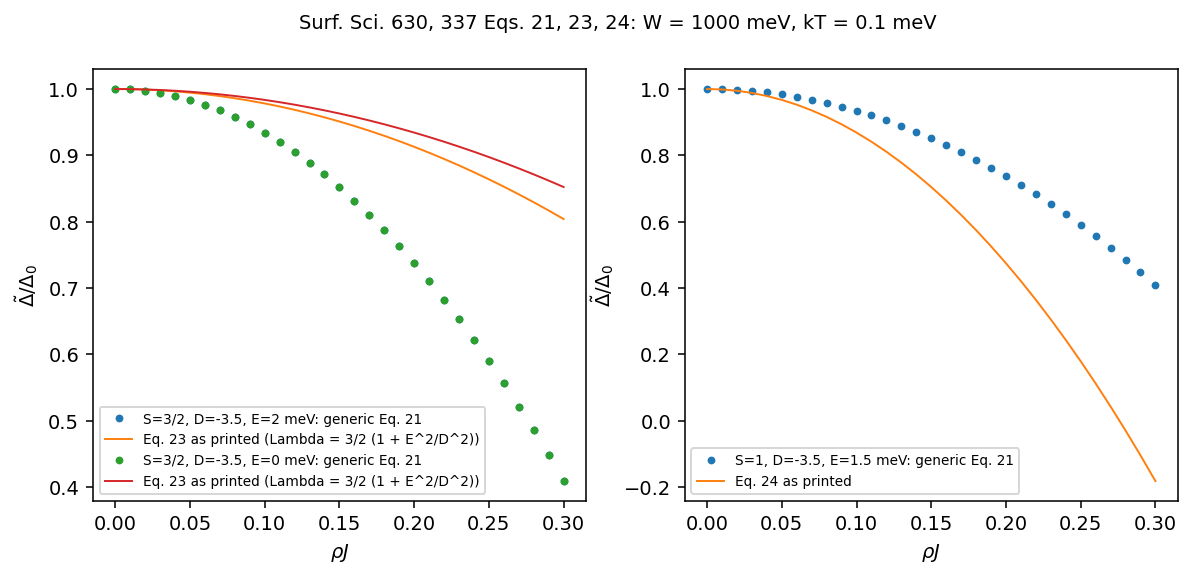
\includegraphics[width=0.48\textwidth]{fig_surfsci_shift.png}
\caption{Surf.\ Sci.: слева $G(\Delta)$ и скорость общего кода; справа сдвиг энергии возбуждения
(ур.~21 против напечатанных ур.~23, 24).}
\label{fig:surf}
\end{figure}

\begin{table}[h]
\centering\small
\begin{tabular}{lr}
\toprule
Сравнение & max.\ откл. \\
\midrule
PRB рис.~2(b): $1-K_d$, ур.~(28), (31)--(32) & $5.6\cdot 10^{-16}$ \\
PRB рис.~2(c): $1+K_d$, ур.~(30), (33)--(34) & $6.7\cdot 10^{-16}$ \\
PRB рис.~3: скорости SW1, SW2 против $\sum K_{ll'}C_lC_{l'}$ & $4.4\cdot 10^{-15}$ \\
PRB ур.~(37): $\Gamma_{SW1}(N)/\Gamma_{SW1}(1)=N$ & $8.0\cdot 10^{-15}$ \\
PRB: $\Lambda^{FM,AFM}$, ED против суммы по ядру, $N=2..8$ & $5.7\cdot 10^{-14}$ \\
PRB ур.~(C3), (C5), (C6 исправл.) против суммы ур.~(16) & $1.5\cdot 10^{-11}$ \\
PRB ур.~(C4) как напечатано против инвариантной суммы & $2.0\cdot 10^{-11}$ \\
SS ур.~(15): $G(\Delta)$ против квадратуры & $2.6\cdot 10^{-13}$ \\
SS ур.~(21) против независимого расчёта той же суммы & $2.2\cdot 10^{-16}$ \\
SS ур.~(24) с коэффициентом $3/4$ вместо напечатанного $3/2$ & $3.3\cdot 10^{-16}$ \\
\midrule
\multicolumn{2}{l}{\emph{расхождения, а не совпадения}} \\
SS ур.~(24) как напечатано & 0.59 \\
SS ур.~(23) как напечатано, $E=0$ и $E=2$ мэВ & 0.44 \\
PRB рис.~4: инвариантная форма против ур.~(16), $\Lambda^{FM}/N^2$ & 1.10 \\
PRB рис.~4: инвариантная форма против ур.~(16), $\Lambda^{AFM}$ & 0.53 \\
\bottomrule
\end{tabular}

\caption{Максимальные отклонения (\texttt{deviations\_*.csv}); таблица собрана скриптом.}
\label{tab:dev}
\end{table}

\paragraph{Сравнение с напечатанными кривыми.}\label{sec:digitize}
Рис.~2(b, c) и~4 PRB оцифрованы из встроенных в PDF изображений
(\path{digitize_reference.py}): кривые выделены по цвету (чёрная --- 1D, красная --- 2D, синяя --- 3D),
для каждого столбца пикселей берётся среднее положение выделенных точек, если их разброс по вертикали
меньше 12 пикселей; вставки и подписи закрыты масками. Погрешность оцифровки видна на кривых, которые
согласуются с формулами (рис.~2(b) 1D и 2(c)): медианное отклонение 0.001, 95-й процентиль $\le0.004$.
Для рис.~4 длина цепочки взята как $N=\mathrm{round}(x/0.01)$ с чётностью панели (ближайшее нужное $N$), что сдвигает
$x$ не более чем на 0.01. Таблица~\ref{tab:digitize}: медиана и 95-й процентиль $|$отклонения$|$ напечатанной
кривой от кандидатной формулы.

\begin{figure}[!htb]
\centering
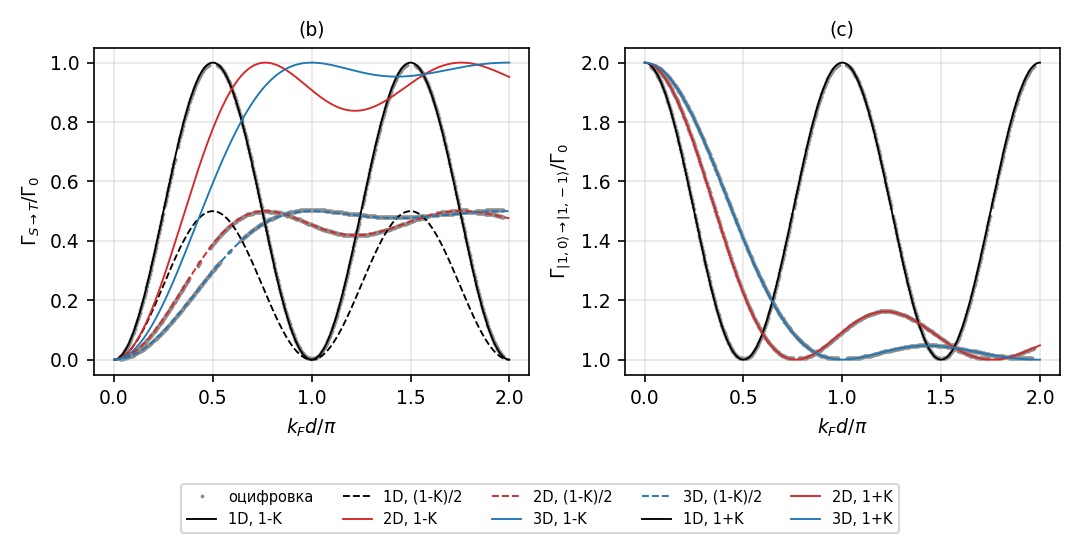
\includegraphics[width=0.85\textwidth]{cmp_fig2.png}
\caption{PRB рис.~2(b, c): серые точки --- оцифровка напечатанных кривых (воспроизведение данных из рисунка
F.~Delgado, J.~Fern\'andez-Rossier, Phys.\ Rev.\ B \textbf{95}, 075413 (2017) \cite{delgado2017}); линии ---
наш расчёт: $1-K_d$ (сплошные), $(1-K_d)/2$ (пунктир) и $1+K_d$ (панель (c)).}
\label{fig:cmp2}
\end{figure}

\begin{figure}[!t]
\centering
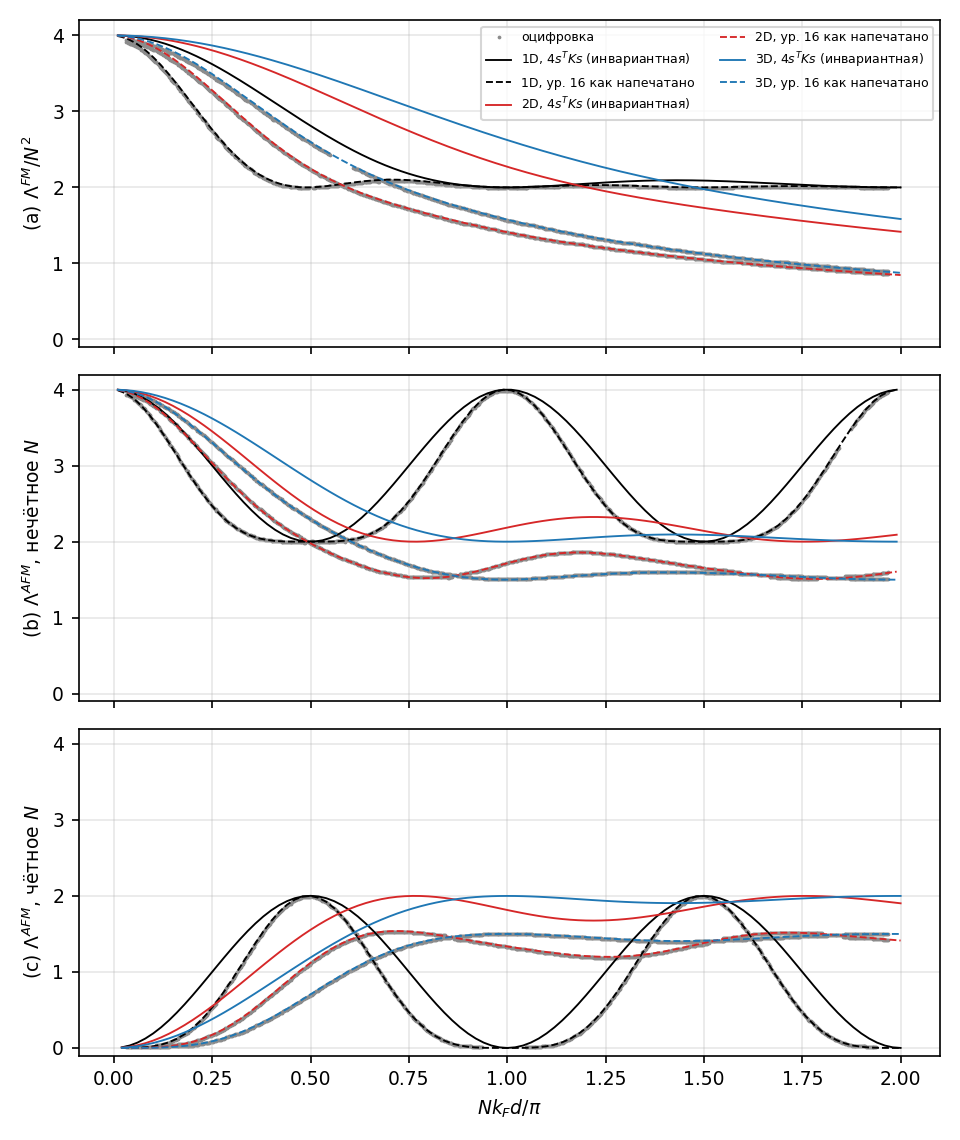
\includegraphics[width=0.72\textwidth]{cmp_fig4.png}
\caption{PRB рис.~4: серые точки --- оцифровка напечатанных кривых (воспроизведение данных из рисунка
F.~Delgado, J.~Fern\'andez-Rossier, Phys.\ Rev.\ B \textbf{95}, 075413 (2017) \cite{delgado2017}); сплошные
линии --- $4s^TKs$, пунктир --- ур.~16 как напечатано. Цвета: чёрный 1D, красный 2D, синий 3D.}
\label{fig:cmp4}
\end{figure}

\begin{table}[h]
\centering\small
\begin{tabular}{llcc}
\toprule
Кривая & & формула 1 & формула 2 \\
\midrule
\multicolumn{4}{l}{\emph{рис.~2: формула 1 --- $1-K_d$ (в (c): $1+K_d$), формула 2 --- $(1-K_d)/2$}} \\
(b) & 1D & 0.001 / 0.003 & 0.242 / 0.490 \\
(b) & 2D & 0.449 / 0.499 & 0.001 / 0.003 \\
(b) & 3D & 0.476 / 0.496 & 0.003 / 0.004 \\
(c) & 1D & 0.001 / 0.003 & -- \\
(c) & 2D & 0.001 / 0.004 & -- \\
(c) & 3D & 0.001 / 0.004 & -- \\
\midrule
\multicolumn{4}{l}{\emph{рис.~4: формула 1 --- $4s^TKs$, формула 2 --- ур.~16 как напечатано}} \\
(a) & 1D & 0.076 / 1.050 & 0.013 / 0.040 \\
(a) & 2D & 0.741 / 1.097 & 0.005 / 0.042 \\
(a) & 3D & 0.866 / 1.108 & 0.006 / 0.040 \\
(b) & 1D & 0.265 / 0.521 & 0.015 / 0.064 \\
(b) & 2D & 0.475 / 0.510 & 0.007 / 0.036 \\
(b) & 3D & 0.494 / 0.512 & 0.005 / 0.030 \\
(c) & 1D & 0.310 / 0.529 & 0.018 / 0.065 \\
(c) & 2D & 0.480 / 0.517 & 0.009 / 0.028 \\
(c) & 3D & 0.501 / 0.510 & 0.008 / 0.023 \\
\bottomrule
\end{tabular}

\caption{Медиана / 95-й процентиль $|$напечатанная кривая $-$ формула$|$ (\texttt{numbers\_digitize.json}).
Шкалы: рис.~2(b) 0--1, 2(c) 1--2, рис.~4 0--4.}
\label{tab:digitize}
\end{table}

\subsection{Расхождения с напечатанным в статьях}

Сравнение со статьёй Surf.\ Sci.\ сделано по препринт-версии. Полные выкладки к каждому пункту --- приложение~\ref{sec:kd}.

\begin{enumerate}[label=(\roman*)]
\item \textbf{PRB рис.~2(b).} Напечатанные кривые 2D и 3D равны половине ур.~31--32:
$(1-J_0^2)/2$ и $(1-\mathrm{sinc}^2)/2$. По оцифровке (наш рис.~\ref{fig:cmp2}, табл.~\ref{tab:digitize})
медианное отклонение от $(1-K)/2$ 0.001 (2D) и 0.003 (3D), от самих ур.~31--32 --- 0.45 и 0.48. Кривая 1D
панели (b) согласуется с $1-K_1$ (медиана 0.001) и не согласуется с половиной (0.24); все три кривые панели (c)
согласуются с $1+K_d$ (медиана 0.001). Матричные элементы дают ур.~31--32; наша панель (b) следует им.
\item \textbf{PRB рис.~4.} Рисунок построен по ур.~16 как напечатано (узлы $r_l=ld$): по оцифровке
(наш рис.~\ref{fig:cmp4}, табл.~\ref{tab:digitize}) медианное отклонение 0.005--0.018 на шкале 0--4 для
всех девяти кривых, против 0.08--0.50 для инвариантной формы $4s^TKs$. После усреднения по поверхности
Ферми ур.~16 даёт
$2\sum s_ls_{l'}[K(k_F|r_l-r_{l'}|)+K(k_F|r_l+r_{l'}|)]$, то есть зависит от выбора начала координат.
Для одного спина ур.~16 даёт $2[1+K(2k_Fr_1)]$, а ур.~38--39 --- 4. Приложение~B (ур.~B2, B3, B6)
содержит только $r_n-r_{n'}$; наша форма $4s^TKs$ инвариантна. Оба варианта совпадают при
$k_Fd\to0$ ($4N^2$ для FM) и имеют период $\pi$ в 1D; различие до 1.1 в $\Lambda^{FM}/N^2$ и 0.53 в $\Lambda^{AFM}$.
\item \textbf{PRB ур.~C4}, а также суммы AFM для 2D и 3D, как напечатано, содержат аргумент
$\xi|l-l'|$ в обоих слагаемых, то есть являются инвариантной суммой, а не напечатанным рисунком. По
ур.~C1 второе слагаемое должно содержать $\xi(l+l')$ ($\xi=k_Fd$).
\item \textbf{PRB ур.~C6} (нечётное $N$) как напечатано не совпадает с суммой ур.~C1 самой статьи и не
стремится к 4 при $k_Fd\to0$. Сумма по C1:
$\tfrac12\big[4+\big(1+\cos((2N+1)\xi)/\cos\xi\big)^2\big]$ (отклонение $\le1.6\cdot10^{-12}$).
\item \textbf{SS ур.~23, 24.} Ур.~21 даёт $\tilde\Delta/\Delta=1-\tfrac34(\rhoJ)^2\ln(2W/\pi\kT)$ для любой
квадратичной анизотропии и спина (проверено для $S=1,\tfrac32,2,\tfrac52$). Ур.~24 печатает $3/2$
(множитель 2); ур.~23 печатает $\Lambda/8$ с $\Lambda=\tfrac32(1+E^2/D^2)$, то есть $3/16$ при $E=0$
(множитель 4); численно $\Lambda=3/2$ при $E=0$ и $E=2$ мэВ. Отклонение напечатанных формул от ур.~21 при $\rhoJ\le0.3$:
0.59 (ур.~24), 0.44 и 0.40 (ур.~23, $E=0$ и $2$ мэВ). Для $W=1$ эВ, $\kT=0.1$ мэВ и уменьшения щели
на 10 мэВ нужно $\rhoJ=0.28$ по общей формуле и 1.4 по ур.~23.
\item \textbf{Префактор.} SS ур.~14 имеет $\pi/2$, PRB ур.~20 --- $\pi/4$; вероятно, разные
соглашения для $\rho$ (не проверялось). Зависит только абсолютный масштаб, не отношения.
\end{enumerate}

\subsection{Демонстрация на двух кубитах}\label{sec:demo}

Скрипт \path{paper/report_2026-11/kondo_demo.py}; рецепты из \texttt{src.blocks}, начальные состояния ---
\texttt{initial.random\_pure}. Параметры: $\rhoJ=0.1$, $\kT=0.2$, $k_F=1$, $J=0.8$, $t_{\max}=1200$,
$dt=1$, порог $1/e$; XXZ и TFIM; $d=1,2,3$; $k_Fd/\pi\in\{0,0.25,\dots,2\}$ (9 точек); $n=30$ случайных
чистых начальных состояний на точку (для всех точек одной системы одни и те же, сид 2026): 1620 траекторий,
59 с на 6 процессах (\path{numbers_kondo_demo.json}). Мера --- $T_2^E$ (пересечение уровня $1/e$ от начального
значения $l_1$-когерентности в энергетическом базисе). Медиана берётся по всем 30 траекториям, нерасчётные
траектории (не пересекли порог до $t_{\max}$) входят со значением $t_{\max}$; 95\% интервал --- бутстреп
медианы (2000 перевыборок, фиксированный сид). Для $T_2^E$ цензурированных траекторий нет (0 из 810 на
систему).

\begin{figure}[h]
\centering
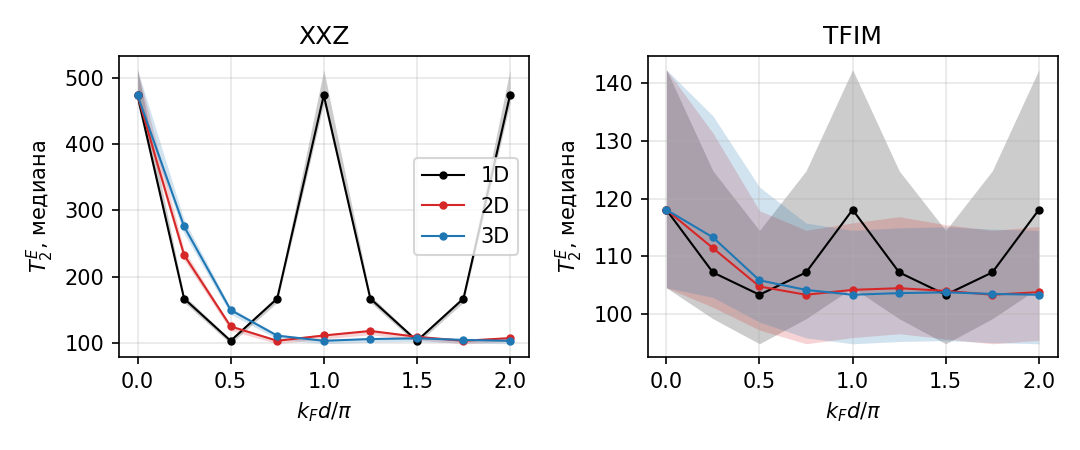
\includegraphics[width=0.9\textwidth]{kondo_demo.png}
\caption{Медиана $T_2^E$ и 95\% бутстреп-интервал против $k_Fd/\pi$ ($n=30$ на точку).}
\label{fig:demo}
\end{figure}

\begin{table}[h]
\centering\small
\begin{tabular}{lccc}
\toprule
$k_Fd/\pi$ & $d=1$ & $d=2$ & $d=3$ \\
\midrule
\multicolumn{4}{l}{\emph{XXZ}} \\
0 & 474 [461, 512] & 474 [461, 512] & 474 [461, 512] \\
0.25 & 167 [162, 172] & 233 [225, 241] & 276 [265, 286] \\
0.5 & 104 [99, 106] & 125 [119, 127] & 150 [144, 154] \\
0.75 & 167 [162, 172] & 104 [99, 106] & 111 [106, 114] \\
1 & 474 [461, 512] & 112 [107, 114] & 104 [99, 106] \\
1.25 & 167 [162, 172] & 118 [113, 120] & 106 [102, 108] \\
1.5 & 104 [99, 106] & 110 [105, 112] & 107 [103, 109] \\
1.75 & 167 [162, 172] & 104 [99, 106] & 105 [100, 107] \\
2 & 474 [461, 512] & 108 [103, 110] & 104 [99, 106] \\
\midrule
\multicolumn{4}{l}{\emph{TFIM}} \\
0 & 118 [105, 142] & 118 [105, 142] & 118 [105, 142] \\
0.25 & 107 [99, 125] & 111 [101, 131] & 113 [103, 134] \\
0.5 & 103 [95, 114] & 105 [97, 118] & 106 [99, 122] \\
0.75 & 107 [99, 125] & 103 [95, 115] & 104 [96, 116] \\
1 & 118 [105, 142] & 104 [96, 116] & 103 [95, 114] \\
1.25 & 107 [99, 125] & 104 [97, 117] & 104 [95, 115] \\
1.5 & 103 [95, 114] & 104 [96, 115] & 104 [95, 115] \\
1.75 & 107 [99, 125] & 103 [95, 114] & 103 [95, 115] \\
2 & 118 [105, 142] & 104 [95, 115] & 103 [95, 114] \\
\bottomrule
\end{tabular}

\caption{Медиана $T_2^E$ [95\% интервал], $n=30$.}
\label{tab:demo}
\end{table}

\begin{itemize}
\item \textbf{XXZ.} Медиана $T_2^E$ от 103.6 до 473.5, в 4.57 раза. Для $d=1$ зависимость периодична
по $k_Fd/\pi$ с периодом 1 (ядро $\cos^2(k_Fd)$): 474 при $k_Fd/\pi=0,1,2$ и 104 при $0.5,1.5$. Для $d=2$: 474 при
$k_Fd=0$, 125 при 0.5 и 104--118 при $k_Fd/\pi\ge0.75$; для $d=3$: 276, 150 и 104--111 (при $0.25$, $0.5$ и
$\ge0.75$). Ширина 95\% интервала 6--11\% медианы.
\item \textbf{TFIM.} Медиана от 103.3 до 118.1, в 1.14 раза; 95\% интервалы (ширина 19--32\% медианы; например, [105, 142]
при $k_Fd=0$ и [95, 114] при $k_Fd/\pi=0.5$, $d=1$) перекрываются, так что зависимость от $k_Fd$ при $n=30$
не разрешена.
\item \textbf{$T_2$ в вычислительном базисе} (те же состояния). Определена плохо: для XXZ 484 из 810
траекторий цензурированы, медиана равна $t_{\max}$ в 22 из 27 ячеек; для TFIM цензурировано 60 из 810 (5
ячеек из 27: $k_Fd=0$ при всех $d$ и целые $k_Fd/\pi$ при $d=1$), медианы 133--923. Для XXZ причина ---
стационарное состояние: при $\kT=0.2$ гиббсово состояние практически синглет (щель 3.2), его
$l_1$-когерентность в вычислительном базисе равна 1, а порог $C_0/e$ ниже 1 у 79\% случайных чистых
начальных состояний (4000 состояний, отдельная проверка), так что такая траектория может пересечь порог
только до релаксации. Для TFIM у гиббсова состояния $l_1=0.37$, ниже порога при любом начальном
состоянии; там цензурирование связано с медленным затуханием в отдельных точках. Это ещё один довод за
цель $T_2^E$. Значения в \path{numbers_kondo_demo.json} (\texttt{t2}) приведены как есть.
\end{itemize}

Ограничения: сдвиг уровней (Lamb shift) в динамику не включён; секулярное приближение (запас для TFIM около
порядка, п.~\ref{sec:model}); $\rhoJ$ постоянно, если не добавлен модификатор $\gamma(t)$; один
выбор $J$, $\kT$, $\rhoJ$; случайные чистые начальные состояния, а не выделенные.

\subsection{Что это даёт проекту}

$T_2^E$ определяется микроскопическими параметрами ($\rhoJ$, $\kT$, $k_Fd$) и для XXZ меняется в 4.6 раза
при изменении $k_Fd/\pi$ от 0 до 0.5 при $d=1$ (474 и 104); для TFIM зависимость слабая (в 1.14 раза). Это
сценарий, в котором предсказываемая цель зависит от скрытого параметра среды (расстояние
$k_Fd$ между спинами), а не от феноменологической $\gamma(t)$. Профиль $\gamma(t)$ и модуляцию OU можно
наложить поверх каналов Кондо тем же рецептом.

\subsection{Выводы по разделу}
\begin{enumerate}
\item \textbf{Модель ванны реализована и проверена.} Скорости переходов и дефазировки в коде совпадают с
  формулами статей; динамика симулятора воспроизводит их с точностью $10^{-14}$.
\item \textbf{Статья I (один спин) воспроизведена.} Закон Корринги и общая формула сдвига уровней совпадают с
  расчётом. Частные формулы сдвига (ур.~23, 24) с общей формулой той же статьи не согласуются: коэффициент
  $3/4$ против напечатанных $3/2$ и $3/16$.
\item \textbf{Статья II (несколько спинов) воспроизведена.} Формулы для димера, спиновых волн и изинговских
  цепочек совпадают с расчётом до машинной точности. На рис.~2(b) кривые 2D и 3D в два раза меньше формул
  статьи; рис.~4 построен по формуле, зависящей от выбора начала координат. Мы следуем формулам,
  согласованным с остальной статьёй.
\item \textbf{Модель применена к задаче проекта.} Ванна Кондо стоит в симуляторе вместо феноменологической
  $\gamma(t)$ для тех же двух кубитов и той же цели.
\item \textbf{Для XXZ время декогеренции зависит от расстояния между кубитами:} $T_2^E$ меняется в 4.6 раза и
  осциллирует с периодом $\pi$ по $k_Fd$; эффект надёжно разрешён (интервалы 6--11\%).
\item \textbf{Для TFIM зависимость слабая} (в 1.14 раза) и при 30 начальных состояниях на точку не разрешена.
\item \textbf{Цель $T_2^E$ лучше, чем $T_2$ в вычислительном базисе:} для XXZ последнее плохо определено из-за
  почти синглетного стационарного состояния.
\item \textbf{Приближения выполнены:} слабая связь ($\rhoJ=0.1$) и секулярное приближение (для TFIM с запасом
  около порядка).
\item \textbf{Следующий шаг:} обучить модели прогноза $T_2^E$ по окну наблюдений при неизвестном $k_Fd$;
  добавить в динамику сдвиг уровней и сравнить с несекулярным уравнением.
\end{enumerate}

\section{Модель наблюдения: конечное число повторов}

Замечание~1 письма: входы --- точные ансамблевые средние. В блоке \path{observe.finite_shots} для
каждого базиса и момента времени из $\rho(t)$ считаются вероятности исходов, разыгрывается
мультиномиальная выборка из $N$ повторов, среднее --- выборочное среднее собственных значений:
\begin{equation}
\hat m_a=\frac{n_+-n_-}{N},\qquad \mathbb E\hat m_a=\langle\sigma_a\rangle,\qquad
\mathrm{Var}\,\hat m_a=\frac{1-\langle\sigma_a\rangle^2}{N}.
\end{equation}
Настройки: \texttt{local} --- 3 базиса ($x,y,z$ для обоих кубитов), даёт шесть локальных средних;
\texttt{tomography} --- $3^n$ базисов (для двух кубитов 9), добавляет корреляторы
$\langle\sigma_a\sigma_b\rangle$. Матрица $\hat\rho$ по линейной инверсии
$\hat\rho=\tfrac1{2^n}\sum \hat m_{\mu}\sigma_\mu$ даёт чистоту и $l_1$-когерентность оценки. Для двух кубитов
они доступны только при томографии (ответ на замечание~2). Стоимость набора: $N\times$(число
настроек)$\times$(число моментов окна); например $N=1000$, 9 настроек, 50 моментов --- $4.5\cdot10^5$
повторов (арифметика, не результат).

\paragraph{Томография.} Томография состояния --- восстановление $\rho$ по средним значениям, полученным
из повторных приготовлений и измерений в разных базисах. Для одного кубита
$\rho=\tfrac12(I+\langle\sigma_x\rangle\sigma_x+\langle\sigma_y\rangle\sigma_y+\langle\sigma_z\rangle\sigma_z)$, и достаточно
трёх настроек измерения. Для двух кубитов матрица $4\times4$ задаётся пятнадцатью средними: шестью
локальными $\langle\sigma_a^{(1)}\rangle$, $\langle\sigma_a^{(2)}\rangle$ и девятью корреляторами
$\langle\sigma_a^{(1)}\sigma_b^{(2)}\rangle$, $a,b\in\{x,y,z\}$; для них нужны девять настроек (каждый кубит в
своём базисе). Когерентность и чистота двух кубитов зависят от корреляторов, поэтому шести локальных
средних для них недостаточно: например, у синглета и полностью смешанного состояния все шесть
локальных средних равны нулю, а чистота равна 1 и $1/4$. Линейная инверсия при конечном $N$ может
дать $\hat\rho$ с отрицательными собственными значениями; отсюда смещение оценок чистоты вверх
(табл.~\ref{tab:bias}).

Сценарий B (один кубит, $\sigma_-$, $\gamma(t)$ в виде полинома Бернштейна, $\omega=1.594$, $t_{\max}=20$,
$dt=0.1$, начальное состояние из сида 5; $\langle\boldsymbol\sigma\rangle_0=(0.908,0.412,0.074)$).

\begin{figure}[h]
\centering
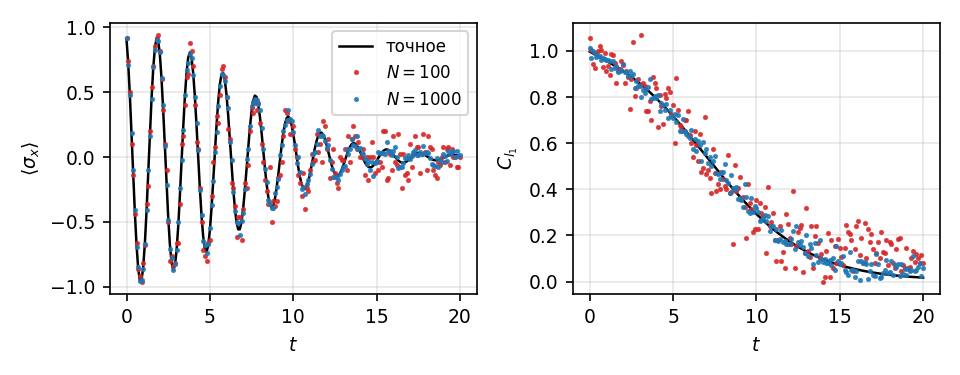
\includegraphics[width=0.95\textwidth]{fig_shots_series.png}
\caption{Точные и оцененные по $N=100$ и $N=1000$ повторам $\langle\sigma_x\rangle(t)$ и
$C_{l_1}(t)$ (одна реализация, фиксированный сид).}
\end{figure}

Среднеквадратичное отклонение оценки от точного ряда по сетке времени: $\sigma_x$ 0.0896 ($N=100$) и 0.0288
($N=1000$); $C_{l_1}$ 0.0835 и 0.0287.

Проверка формулы дисперсии: 2000 повторений при фиксированных сидах на шести моментах времени
(табл.~\ref{tab:std}). По всем осям отклонение эмпирической std от $\sqrt{(1-m^2)/N}$ не более 4.1\%
(ожидаемая погрешность самой эмпирической std 1.6\%); исключены две пары (ось, момент) с
$|m|\ge0.99$, где распределение дискретно.

\begin{table}[h]
\centering\small
\begin{tabular}{rrrrrr}
\toprule
& & \multicolumn{2}{c}{$N=100$} & \multicolumn{2}{c}{$N=1000$} \\
\cmidrule(lr){3-4}\cmidrule(lr){5-6}
$t$ & $\langle\sigma_x\rangle$ & эмпир. & $\sqrt{(1-m^2)/N}$ & эмпир. & $\sqrt{(1-m^2)/N}$ \\
\midrule
0 & 0.908 & 0.0411 & 0.0419 & 0.0132 & 0.0132 \\
2 & 0.792 & 0.0610 & 0.0610 & 0.0189 & 0.0193 \\
5 & -0.566 & 0.0834 & 0.0824 & 0.0259 & 0.0261 \\
10 & 0.183 & 0.0990 & 0.0983 & 0.0316 & 0.0311 \\
15 & -0.030 & 0.0993 & 0.1000 & 0.0312 & 0.0316 \\
20 & 0.003 & 0.0988 & 0.1000 & 0.0314 & 0.0316 \\
\bottomrule
\end{tabular}

\caption{Эмпирическая std оценки $\hat m_x$ против $\sqrt{(1-m^2)/N}$, 2000 повторений.}
\label{tab:std}
\end{table}

Оценки чистоты и $C_{l_1}$ из $\hat\rho$ смещены: $\mathbb E P=\tfrac12(1+|\mathbf r|^2+(3-|\mathbf r|^2)/N)$,
то есть $\Delta P=(3-|\mathbf r|^2)/2N$; для $C_{l_1}=\sqrt{\hat m_x^2+\hat m_y^2}$ смещение положительно
и растёт, когда истинная когерентность мала (табл.~\ref{tab:bias}). Максимальное расхождение $\Delta P$
с формулой --- 2.6 стандартной ошибки из 12 сравнений.

\begin{table}[h]
\centering\small
\begin{tabular}{rrrrrr}
\toprule
& \multicolumn{3}{c}{$N=100$} & \multicolumn{2}{c}{$N=1000$} \\
\cmidrule(lr){2-4}\cmidrule(lr){5-6}
$t$ & $\Delta P$ & $(3-|\mathbf r|^2)/2N$ & $\Delta C_{l_1}$ & $\Delta P$ & $\Delta C_{l_1}$ \\
\midrule
0 & +0.0125 & 0.0100 & +0.0065 & +0.00068 & +0.00011 \\
2 & +0.0110 & 0.0108 & +0.0044 & +0.00059 & +0.00000 \\
5 & +0.0093 & 0.0114 & +0.0041 & +0.00061 & -0.00009 \\
10 & +0.0102 & 0.0105 & +0.0169 & +0.00193 & +0.00218 \\
15 & +0.0102 & 0.0100 & +0.0721 & +0.00096 & +0.00731 \\
20 & +0.0101 & 0.0100 & +0.1101 & +0.00098 & +0.02552 \\
\bottomrule
\end{tabular}

\caption{Смещение оценок чистоты ($\Delta P$) и $l_1$-когерентности ($\Delta C_{l_1}$).}
\label{tab:bias}
\end{table}

\textbf{Влияние на точность предсказателей (пункт B, «точность против стоимости набора») не
посчитано.}

\section{Записи последовательных измерений}

Направление C. Протокол (\path{evolve.sequential_record}): измерение в $t_0$; между
моментами эволюция по уравнению Линдблада; проективное измерение $\sigma_z$, исход по вероятностям Борна,
коллапс на исход. Исход 0 соответствует $\sigma_z=+1$. Две проверки на $10^3$--$4\cdot10^3$ записей
(тесты того же в \path{tests/unit/blocks/test_evolve.py}; здесь большая выборка), $dt=0.5$, $t_{\max}=6$.

\begin{figure}[h]
\centering
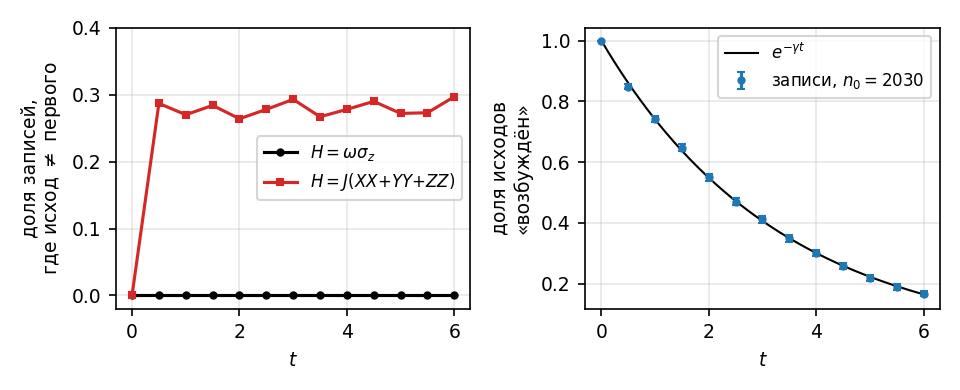
\includegraphics[width=0.95\textwidth]{fig_records.png}
\caption{(a) Эффект Зенона: при $H=\omega\sigma_z$ и без диссипации исходы не меняются; для
$H=J(XX+YY+ZZ)$ меняются. (b) Затухание амплитуды, $\gamma=0.3$: доля возбуждённых исходов среди записей
с первым исходом 0, биномиальные ошибки.}
\end{figure}

\begin{enumerate}[label=(\alph*)]
\item Зенон: из 12000 проверенных исходов (1000 записей) изменений 0. Контраст при XXZ: доля записей с исходом,
отличным от первого, в среднем 0.279 при $t\ge1$.
\item Затухание амплитуды: $n_0=2030$ из 4000 записей с первым исходом 0; после коллапса $p_0=1$, и доля
возбуждённых равна $e^{-\gamma t}$ (табл.~\ref{tab:rec}). Наибольшее $|z|$ среди 12 моментов 1.55;
из 1970 записей с первым исходом 1 ни одна не вернулась в возбуждённое состояние.
Точки одной выборки коррелированы, $\chi^2$ не считался.
\end{enumerate}

\begin{table}[h]
\centering\small
\begin{tabular}{rrrrr}
\toprule
$t$ & $\hat p(t)$ & $e^{-\gamma t}$ & $\sigma_{\rm bin}$ & $(\hat p-e^{-\gamma t})/\sigma_{\rm bin}$ \\
\midrule
0 & 1.000 & 1.000 & 0.000 & -- \\
1 & 0.742 & 0.741 & 0.010 & +0.11 \\
2 & 0.550 & 0.549 & 0.011 & +0.13 \\
3 & 0.412 & 0.407 & 0.011 & +0.48 \\
4 & 0.301 & 0.301 & 0.010 & -0.02 \\
5 & 0.219 & 0.223 & 0.009 & -0.42 \\
6 & 0.168 & 0.165 & 0.008 & +0.33 \\
\bottomrule
\end{tabular}

\caption{Доля возбуждённых исходов $\hat p(t)$ против $e^{-\gamma t}$.}
\label{tab:rec}
\end{table}

Не сделано: модель на записях, цель, базовая модель по правдоподобию записи а-ля Luchnikov et al.\
\cite{luchnikov2020}.

\section{Программная основа и воспроизводимость}

Блочный конструктор (\texttt{src/blocks}, \path{notes/constructor_design.md} §1) устранил:
\begin{itemize}
\item варианты физики как подклассы симулятора, которые нельзя сочетать (Кондо со стохастической $\gamma$);
\item дисковый кэш только для одного варианта (ключ строился лишь из \texttt{SystemConfig});
\item шум $\gamma$ и начальные состояния, зависящие от порядка вызовов (глобальный \texttt{np.random});
\item симулятор, возвращавший только наблюдаемые и цель: смена цели требовала новой симуляции.
\end{itemize}
Каждая траектория имеет свой поток случайных чисел, зависящий только от (сид, номер). Проверка
опубликованных чисел (\path{scripts.golden_outputs}, 42 записи) не менялась и
после каждого шага рефакторинга даёт те же значения. Кроме того, CSV быстрых прогонов (\texttt{--fast})
сравнивались побайтно (\texttt{cmp}) с результатами кода до изменений: R5, R7, R21, R26 и демо R28 после
перехода на блоки; E1--E8, E11, R2, R17, R18 после чистки экспериментов. Все совпали.

\paragraph{Интерфейс.} В рабочем интерфейсе (\texttt{app.py}) добавлен экран сборки рецепта из блоков
без кода: выбор блоков и параметров по шагам, разброс параметра по траекториям, предпросмотр 1--5
траекторий с графиком и временем до порога, сохранение рецептов и фоновая генерация датасета. Тот же
рецепт запускается из командной строки (\texttt{python -m src.blocks.cli generate}).

\paragraph{Эксперименты.} Скрипты разложены по папкам \texttt{paper1/}, \texttt{paper2/},
\texttt{checks/} (R2, нигде не цитируется) и \texttt{new/} (R28); номера и имена файлов результатов не
менялись. Карта \texttt{experiments/README.md} связывает вопрос, эксперимент, главный результат из CSV и
место цитирования. Нецитируемые E9, E10, E12--E14 удалены (код остаётся в истории git). Старый
дисковый кэш траекторий (1.6 ГБ) удалён: его результат зависел от того, что уже лежало в кэше.

\section{Дальнейшие шаги и вопросы}

\paragraph{Шаги.} (1) Таблица B: точность против стоимости набора. (2) Цель на записях и базовая модель.
(3) Сдвиг уровней (Lamb shift) в динамике ванны Кондо.

\paragraph{Вопросы (из плана, §6, ответов нет).}
\begin{enumerate}
\item Сценарий текущих статей: характеризация и калибровка (ансамблевые входы) после правок A--B, или
подавать только после перехода к последовательным измерениям?
\item Направление C --- продолжение диплома или отдельная (третья) статья?
\item Модель измерений для C: проективные или слабые/непрерывные; какой набор наблюдаемых (например, только $\sigma_z$)?
\item Цель в C: время до порога или параметры среды и генератор?
\end{enumerate}

\appendix
% Вывод формул ванны Кондо и разбор расхождений с напечатанным.
% Подключается в отчёт (report_2026-11/report.tex) и в описание
% (kondo_simulations.tex). Требует в преамбуле \kddir и kondo_boxes.tex.

\section{Вывод формул ванны Кондо и разбор расхождений}
\label{sec:kd}

\input{\kddir kd/part1_rate.tex}
\input{\kddir kd/part2_shift.tex}
\input{\kddir kd/part3_prb.tex}
\input{\kddir kd/part4_conv.tex}


\section{Квантовый отжиг (курс QML)}

Точные симуляции, $N=8$, одна задача Шеррингтона--Киркпатрика (сид 7), \path{../Annealing/qa_figures.py}; числа из
\path{figures/annealing_numbers.json}. Рисунки сделаны для слайдов, без легенд.

\begin{figure}[h]
\centering
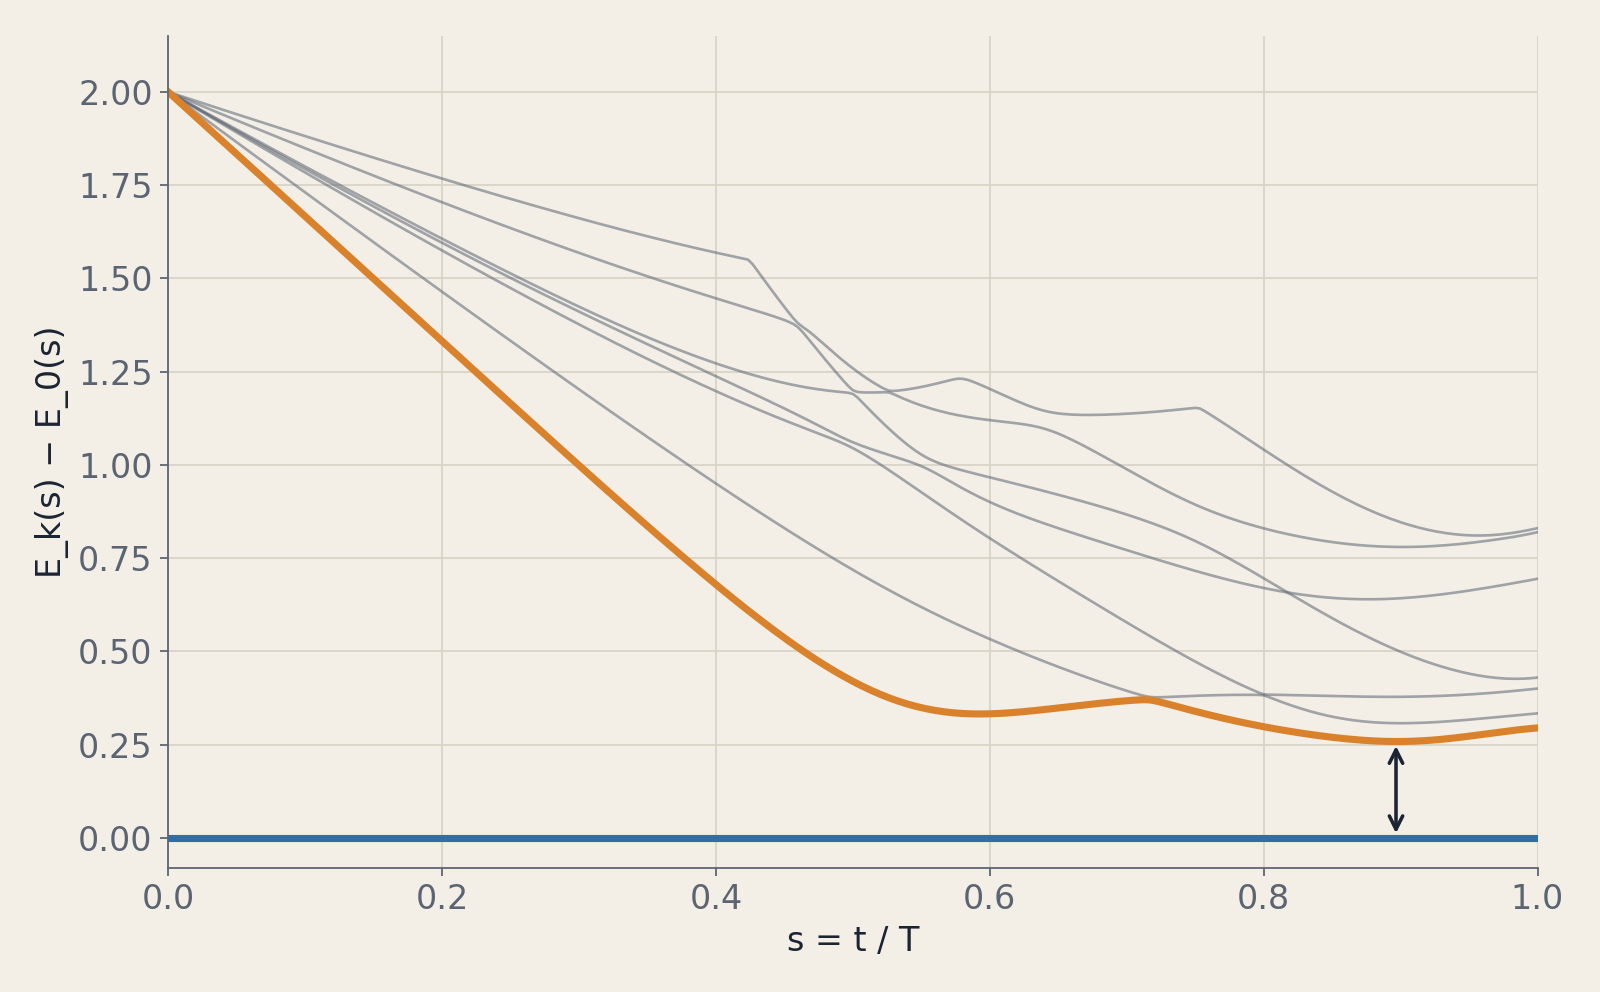
\includegraphics[width=0.48\textwidth]{annealing_spectrum.png}\hfill
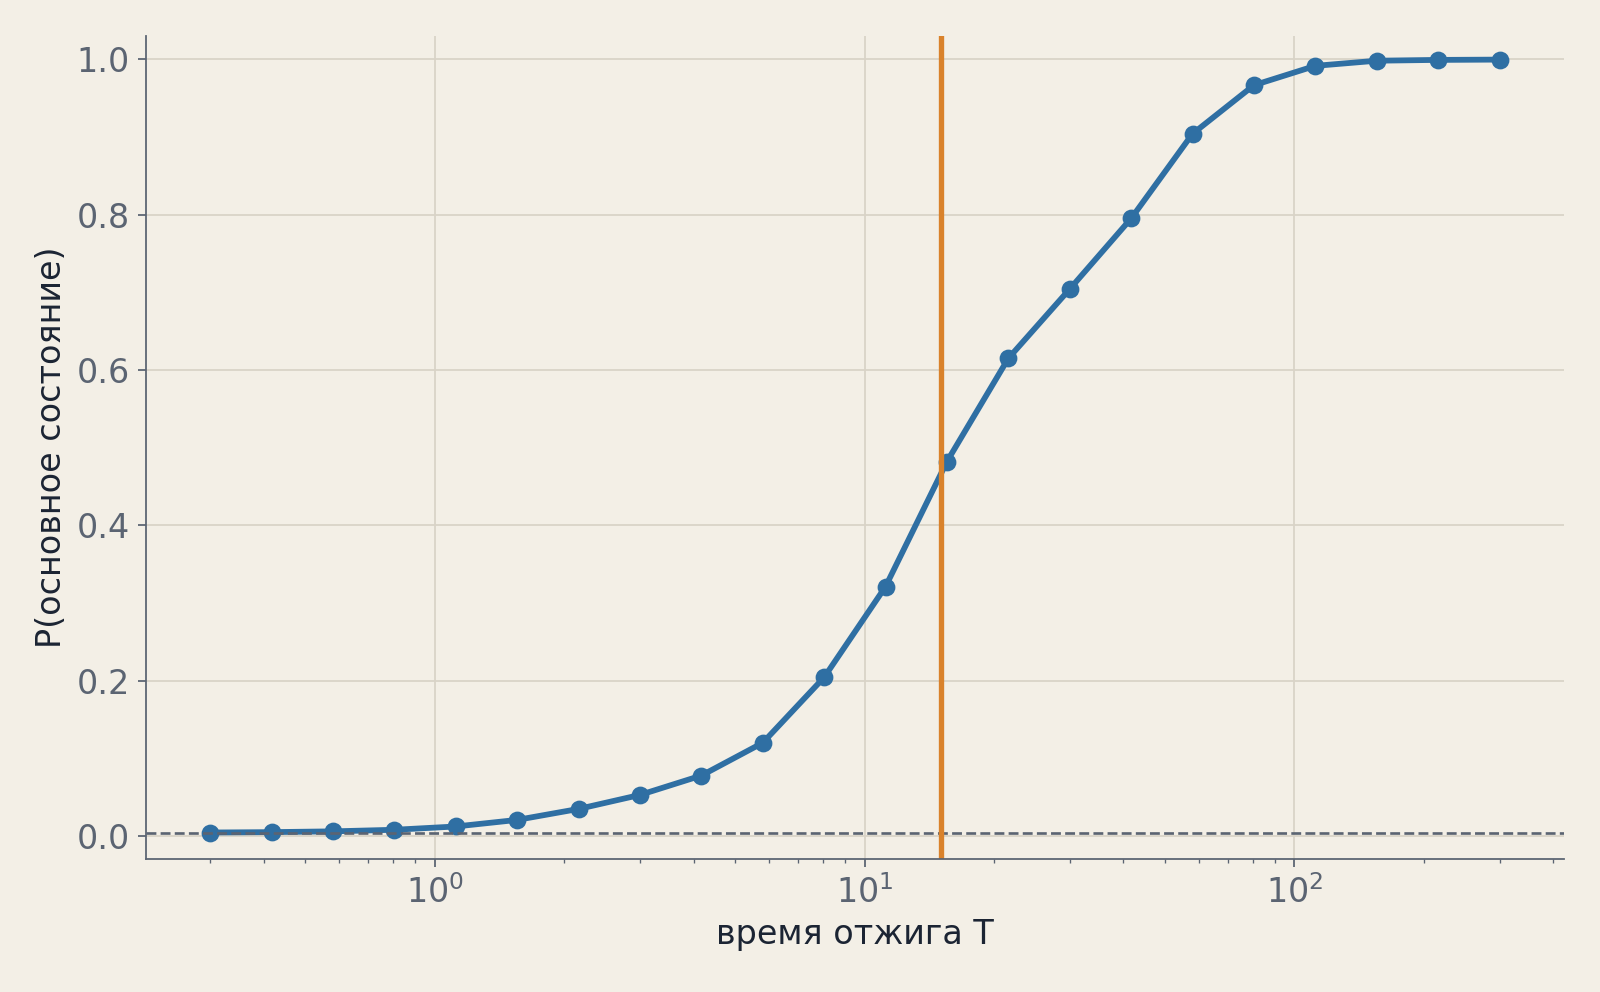
\includegraphics[width=0.48\textwidth]{annealing_p_vs_T.png}\\[4pt]
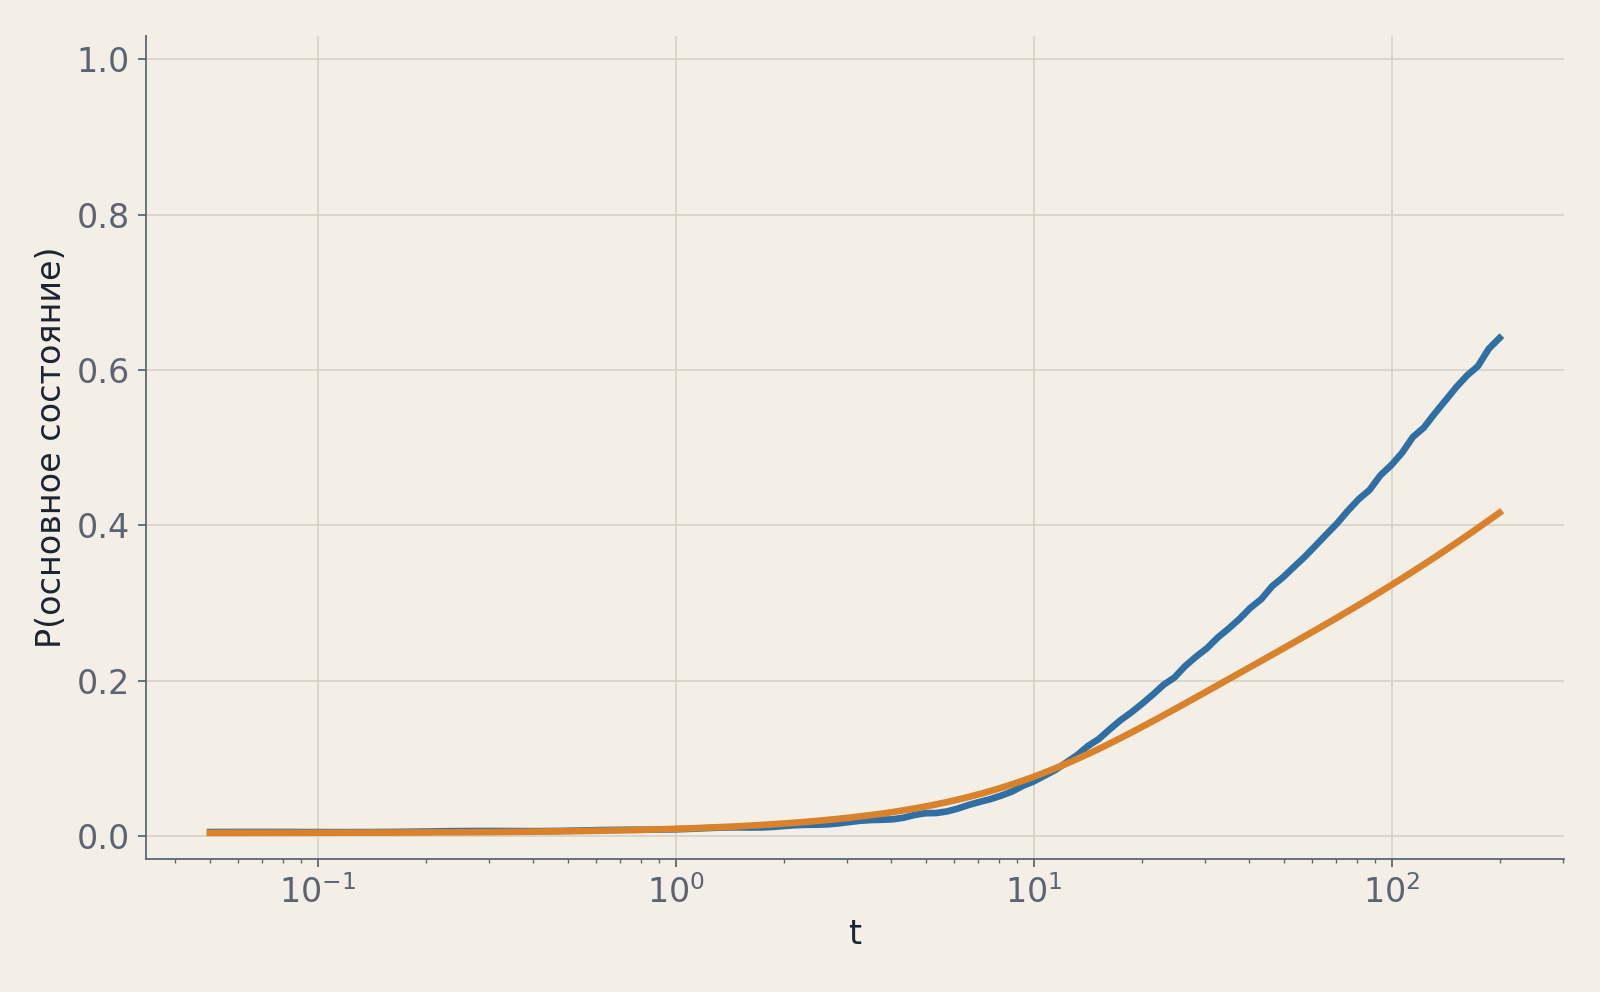
\includegraphics[width=0.48\textwidth]{annealing_kn98.png}\hfill
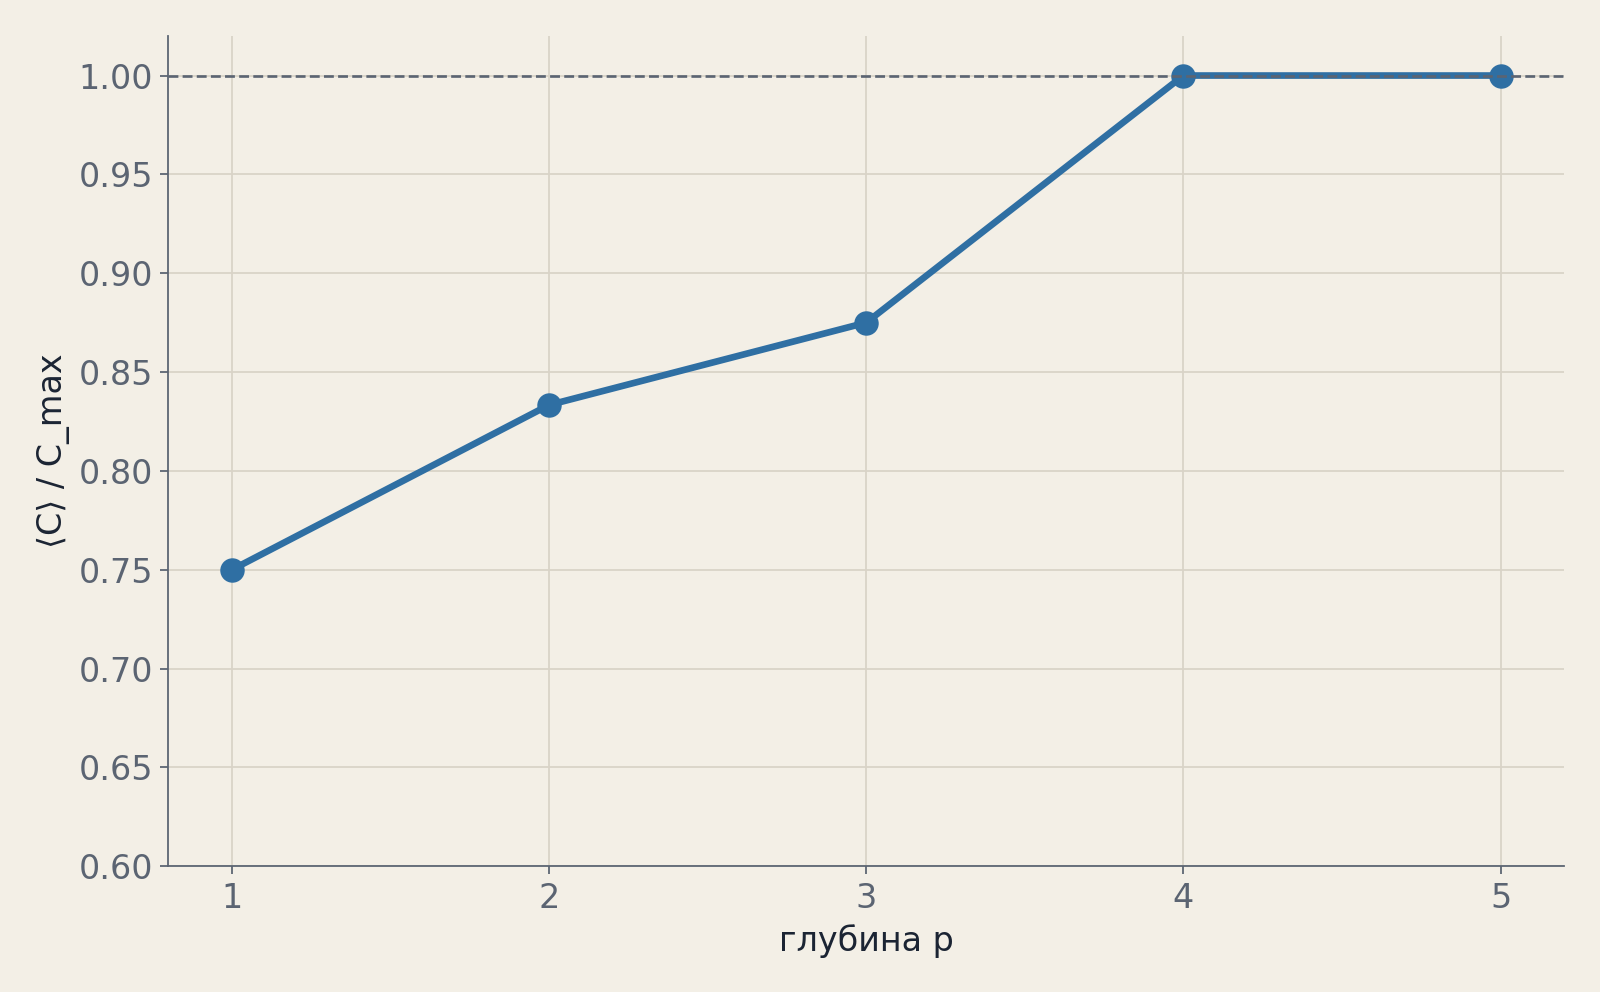
\includegraphics[width=0.48\textwidth]{annealing_qaoa.png}
\caption{Сверху: спектр $H(s)=-(1-s)\sum X+sH_P$ (оранжевый --- первая щель); вероятность основного
состояния от времени отжига $T$. Снизу: $\Gamma(t)=T(t)=3/\sqrt t$, QA (синий) против SA (оранжевый); QAOA на кольце из 8 вершин.}
\end{figure}

\begin{itemize}
\item $E_{gs}=-4.369$; минимальная щель $\Delta_{\min}=0.258$ при $s=0.897$; $1/\Delta_{\min}^2=15.0$.
\item $P(T=15.5)=0.482$; $P(T=57.9)=0.904$; $P(T=300)=0.9996$.
\item Подход Kadowaki--Nishimori \cite{kn98}: при $t=200$ QA 0.641, SA 0.416 (одна реализация).
\item QAOA \cite{farhi2014} (MaxCut, кольцо из 8), $\langle C\rangle/C_{\max}$ при $p=1..5$:
0.75, 0.8333, 0.875, 1.0, 1.0 (округление до 4 знаков).
\end{itemize}

\begin{thebibliography}{9}
\bibitem{delgado2017} F.~Delgado, J.~Fern\'andez-Rossier, Phys.\ Rev.\ B \textbf{95}, 075413 (2017).
\bibitem{delgado2014} F.~Delgado, C.~F.~Hirjibehedin, J.~Fern\'andez-Rossier, Surf.\ Sci.\ \textbf{630}, 337 (2014).
\bibitem{luchnikov2020} I.~A.~Luchnikov, S.~V.~Vintskevich, D.~A.~Grigoriev, S.~N.~Filippov, Phys.\ Rev.\ Lett.\ \textbf{124}, 140502 (2020); arXiv:1902.07019.
\bibitem{teretenkov2026} A.~E.~Teretenkov, Kuznetsov, Pechen, Learning Hidden Structures in Open Quantum Dynamics, arXiv:2604.00711 (2026).
\bibitem{mavadia2017} S.~Mavadia, V.~Frey, J.~Sastrawan, S.~Dona, M.~J.~Biercuk, Nat.\ Commun.\ \textbf{8}, 14106 (2017).
\bibitem{maan2026} Maan et al., Anticipating Decoherence for Enhancing Coherence in Quantum Systems, arXiv:2508.02638.
\bibitem{chenkuo2025} Chen, Kuo, Phys.\ Rev.\ A \textbf{112}, 042227 (2025); arXiv:2505.06928.
\bibitem{napdd2026} Abu-Nada, Banerjee, Wu, Noise-Adaptive Predictive Dynamical Decoupling, arXiv:2606.15769 (2026).
\bibitem{kn98} T.~Kadowaki, H.~Nishimori, Phys.\ Rev.\ E \textbf{58}, 5355 (1998).
\bibitem{farhi2014} E.~Farhi et al., arXiv:1411.4028.
\end{thebibliography}

\end{document}
